\documentclass{article}
\usepackage{graphicx} % Required for inserting images
\usepackage{graphicx}
\usepackage{hyperref}
\usepackage[T1]{fontenc}
\usepackage{listings}
\usepackage{graphicx}
\usepackage{amsmath}
\usepackage[serbian]{babel}


\title{\textbf{Transformers - Text Similarity, Clustering}}
\author{Nikolina Pejović 172/2019,  Jelena Maksimović 193/2018}

\date{Septembar 2024}


\begin{document}

\maketitle

\section{Uvod}

U ovom radu istražujemo primenu transformera, s posebnim fokusom na BERT model, za određivanje sličnosti između rečenica u skupu podataka koji nosi naziv \href{https://huggingface.co/datasets/PhilipMay/stsb_multi_mt}{STSB\_MULTI\_MT}. Ovaj dataset sadrži rečenice koje su anotirane prema stepenu semantičke sličnosti, što predstavlja izazov zbog jezičke raznolikosti i varijabilnosti konteksta. Analizom različitih tehnika generisanja embeddings-a i primenom metoda klasterovanja, cilj nam je da procenimo efikasnost transformera u zadatku procene sličnosti rečenica, čime želimo da doprinesemo što boljem razumevanju njihovih mogućnosti u obradi prirodnog jezika


\section{Transformeri}

Transformeri su napredni modeli za obradu prirodnog jezika koji koriste mehanizam pažnje kako bi efikasno razumeli i generisali tekst. Ovi modeli omogućavaju paralelnu obradu sekvencijalnih podataka, čime se značajno poboljšavaju brzina treniranja i ukupna efikasnost. Sastoje se od višeslojnih kodirajućih i dekodirajućih blokova koji uče složene reprezentacije i odnose među podacima, omogućavajući precizno razumevanje konteksta i semantike.

Transformeri su od ključnog značaja za mnoge savremene aplikacije u veštačkoj inteligenciji, kao što su prevođenje, sažimanje, generisanje i procena sličnosti teksta.

Njihova fleksibilnost i sposobnost prilagođavanja različitim zadacima čine transformere jednim od najvažnijih i najmoćnijih alata u modernom mašinskom učenju.

\subsection{Modeli}


Neki od najpopularnijih modela baziranih na arhitekturi transformera uključuju:

\begin{itemize}
\item\textbf{BERT (Bidirectional Encoder Representations from Transformers)}:
Model fokusiran na razumevanje konteksta reči u oba smera. Koristi se za različite zadatke poput klasifikacije teksta, prepoznavanja entiteta i odgovaranja na pitanja.

\item\textbf{GPT (Generative Pre-trained Transformer)}:
Generativni model osposobljen za kreiranje teksta. Različite verzije, poput GPT-2 i GPT-3, imaju široku primenu u generisanju koherentnog i smislenog teksta u mnogim kontekstima.

\item\textbf{T5 (Text-to-Text Transfer Transformer)}:
Model koji sve NLP zadatke tretira kao probleme prevođenja. Koristi se u zadacima kao što su sažimanje teksta, prevođenje i klasifikacija, čime demonstrira svoju fleksibilnost.

\end{itemize}

\subsection{Treniranje modela}

Na početku, učitavamo potrebne biblioteke, uključujući \textit{transformers}, za rad sa BERT modelom i \textit{datasets}, za upravljanje skupovima podataka. Zatim, koristeći funkciju \textbf{load\_dataset}, učitavamo englesku verziju STS-B dataseta i delimo ga na tri dela: trening, validaciju i test. Ova podela omogućava nam da obučimo model na jednom delu podataka, dok drugi delovi služe za evaluaciju njegove tačnosti i sposobnosti generalizacije.

Nakon toga, prikazujemo nekoliko primera iz trening dataset-a kako bismo dobili uvid u strukturu podataka. U ovom skupu imamo parove rečenica i njihove rezultate sličnosti, što nam pomaže da shvatimo kako model treba da uči. Neki od primera su:

\begin{itemize} 
    \item \textbf{Primer 1:}
    \begin{lstlisting}
{'sentence1': 'A plane is taking off.', 
'sentence2': 'An air plane is taking off.', 
'similarity_score': 5.0}
    \end{lstlisting}
    Ove dve rečenice su vrlo slične, što se odražava u oceni sličnosti 5.0, označavajući da se zapravo radi o istom događaju.
\end{itemize}

\begin{itemize} 
    \item \textbf{Primer 2:}
    \begin{lstlisting}
{'sentence1': 'Three men are playing chess.',
'sentence2': 'Two men are playing chess.',
'similarity_score': 2.59}
    \end{lstlisting}
    Ove rečenice imaju nižu ocenu sličnosti zbog razlike u broju igrača, što može značiti različite situacije.
\end{itemize}

\begin{itemize} 
    \item \textbf{Primer 3:}
    \begin{lstlisting}
{'sentence1': 'A man is playing the cello.',
'sentence2': 'A man seated is playing the cello.',
'similarity_score': 4.25}.
    \end{lstlisting}
    Iako se radi o istoj radnji, dodatak \textit{seated} dodaje kontekst, ali ne umanjuje sličnost između rečenica. 
\end{itemize}

Ovi primeri ilustruju raznolikost u podacima koje model koristi za učenje. Razumevanje ovih odnosa između rečenica i njihovih ocena sličnosti ključno je za pravilno obučavanje modela.

Kada se upoznamo sa podacima, kreiramo BERT tokenizator, koji je ključan za konvertovanje rečenica u formate koje model može obraditi. Definišemo funkciju za tokenizaciju koja obrađuje parove rečenica, primenjujući skraćivanje, dodavanje praznog prostora, i postavljajući maksimalnu dužinu tokena na 128. Nakon tokenizacije, dodajemo oznake koje predstavljaju ocene sličnosti između rečenica.

Da bismo nastavili s obradom, konvertujemo tokenizovane podatke u \textit{Dataset} objekat, koji je potreban za treniranje modela. Kreiramo BERT model za regresiju, postavljajući \texttt{num\_labels=1}, s obzirom na to da se bavimo predikcijom jednog kontinuiranog rezultata — sličnosti između rečenica.

\vspace{1em}
Zatim definišemo argumente za trening, kao što su: \begin{itemize} \item broj epoha, \item veličina batch-a, \item postepena inicijalizacija stope učenja, \item regularizacija težina. \end{itemize}

Ovi parametri igraju ključnu ulogu u optimizaciji procesa učenja i efikasnosti obuke modela, čime se poboljšavaju njegove performanse


Na kraju, kreiramo objekat \textbf{Trainer}, koji uključuje model, definisane argumente za trening, test i validacioni dataset. Pokrećemo proces obuke pozivom metode \textit{trainer.train()}, što omogućava modelu da uči iz podataka i optimizuje svoje težine kako bi precizno procenio sličnost između rečenica.

Kombinovanjem BERT-a i STS-B dataseta, ovaj pristup omogućava nam da istražimo kako modeli zasnovani na transformerima mogu uspešno razumeti složene semantičke odnose u tekstu, čime se otvaraju mogućnosti za različite aplikacije u oblasti obrade prirodnog jezika.

\subsection{Evaluacija modela}
U ovom delu vrši se evaluacija modela i izračunavanje nekoliko metrika koje pomažu u proceni njegove tačnosti u predikciji sličnosti između rečenica. Nakon završetka obuke, pozivamo metodu \textit{trainer.evaluate()}, koja vraća osnovne rezultate evaluacije modela, kao što su gubitak i druge relevantne metrike.

Nakon toga, pristupamo predikciji sličnosti na test dataset-u. Koristimo \textit{trainer.predict(test\_dataset)} da bismo dobili predikcije modela za neviđene podatke. Rezultate zatim konvertujemo u niz kako bismo olakšali dalju obradu. Istovremeno, izdvajamo prave vrednosti (\textit{true\_labels}) iz test dataset-a za poređenje sa predikcijama.

Rezultati evaluacije modela ukazuju na relativno dobre performanse u zadatku procene sličnosti između rečenica.

\newpage
\textbf{2.3.1. \underline{Rezultati evaluacije}:}
\vspace{1em}

\textbf{Eval Loss}:
Gubitak tokom evaluacije iznosi 0.461. Ova vrednost funkcije gubitka meri udaljenost između predikcija modela i stvarnih vrednosti. Niže vrednosti gubitka sugerišu bolje performanse modela. U ovom slučaju, vrednost gubitka ukazuje na to da model generalno dobro predviđa sličnosti, ali postoji prostor za poboljšanje.


\textbf{Eval Runtime}: Evaluacija modela trajala je oko 7.5 sekundi, što ukazuje na brzinu obrade test podataka.


\textbf{Eval Samples per Second}: Model je obradio približno 199.86 uzoraka u sekundi, što ukazuje na dobru brzinu evaluacije

\textbf{Eval Steps per Second}: Model je izveo 25.05 koraka u sekundi. Ove informacije su korisne za procenu efikasnosti modela prilikom rada sa velikim skupovima podataka.

\vspace{1em}
\textbf{2.3.2. \underline{Metrike performansi}:}
\vspace{1em}

\textbf{Mean Absolute Error (MAE)}: Vrednost MAE iznosi 0.611, što sugeriše da je prosečna apsolutna greška između predikcija i stvarnih vrednosti oko 0.61. To znači da, u proseku, model greši za oko 0.61 poen u oceni sličnosti, što se može smatrati razumnim u kontekstu ovog zadatka.

\textbf{Root Mean Squared Error (RMSE)}: RMSE iznosi 0.821, što ukazuje na to da su veće greške teže kažnjene u ovoj metriki. RMSE je nešto viši od MAE, što sugeriše da model može imati nekoliko većih grešaka. Međutim, vrednost ostaje u prihvatljivim granicama.

\textbf{Pearson Correlation Coefficient}: Vrednost od 0.844 ukazuje na vrlo dobar pozitivni linearni odnos između predikcija i stvarnih vrednosti. Ova visoka korelacija sugeriše da model efikasno prepoznaje odnose u podacima u podacima i može pouzdano predviđati sličnosti između rečenica.

\section{Raspodela gresaka}

Dobijen je histogram koji vizualizuje raspodelu grešaka između predikcija modela i stvarnih vrednosti iz test dataset-a. Histogram se generiše korišćenjem biblioteke \textbf{matplotlib}, koja omogućava raznolike načine prikazivanja podataka.

\newpage

\begin{figure}[t]
    \centering 
    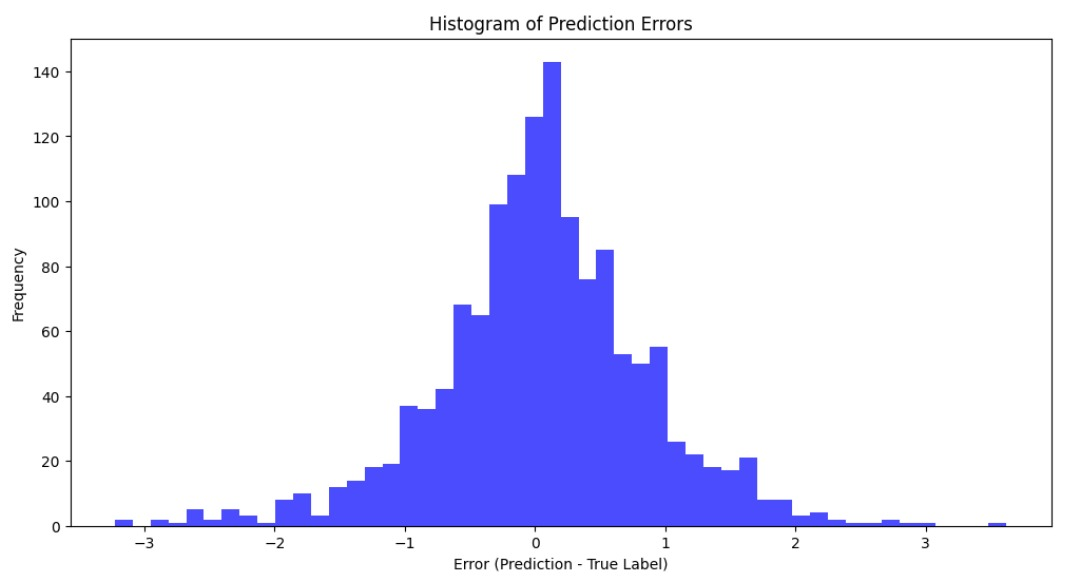
\includegraphics[width=0.8\textwidth]{ri1.jpeg} 
\end{figure}

Na x-osi histogram prikazuje razliku između predikcija i stvarnih vrednosti (grešku), dok y-osa pokazuje učestalost svake greške. Koristimo 50 intervala za detaljniji pregled raspodele grešaka. Histogram je obojen u plavu boju, a stepen prozirnosti (alpha) je postavljen na 0.7, čime se povećava preglednost vizualizacije.

Rezultati prikazani na histogramu ukazuju na to da se najveći deo grešaka nalazi u blizini nulte tačke. Ovo sugeriše da model većinom predviđa sličnosti koje su bliske stvarnim vrednostima, što je pozitivan znak i ukazuje na dobre performanse modela. U isto vreme, manji broj grešaka u ekstremnim vrednostima pokazuje da su velike razlike između predikcija i stvarnih vrednosti relativno retke. Ova distribucija grešaka naglašava stabilnost modela, jer se većina njegovih predikcija nalazi u blizini stvarnih vrednosti, dok su ekstremne greške izuzeci, a ne pravilo.


\begin{figure}[h]
    \centering 
    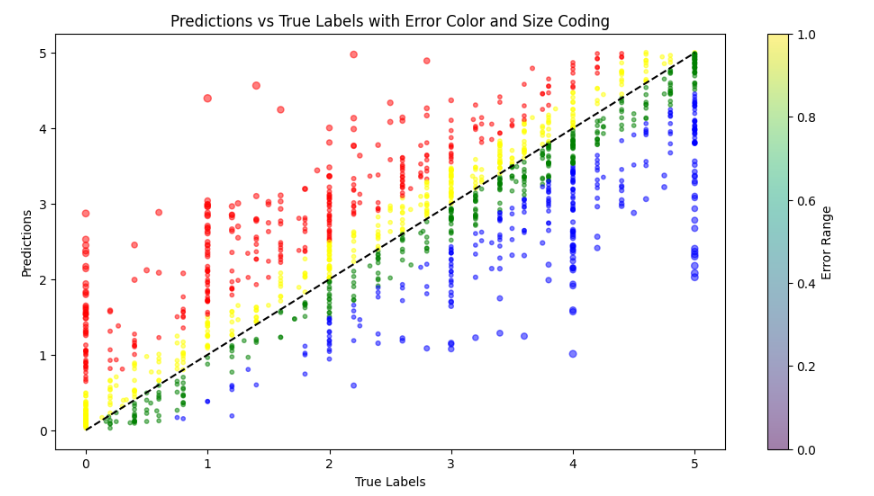
\includegraphics[width=0.8\textwidth]{ri3.png} 
\end{figure}

Ovaj scatter plot prikazuje predikcije modela u poređenju sa stvarnim vrednostima (\textbf{True Labels}). Boje i veličine tačaka na grafikonu odražavaju veličinu grešaka između predikcija i stvarnih vrednosti. Tačke koje su dalje od crne isprekidane linije (predstavlja savršenu tačnost) označavaju veće greške modela.

X osa predstavlja stvarne vrednosti (\textbf{True Labels}), dok Y osa prikazuje predikcije modela (\textbf{Predictions}).

\vspace{1em}
\textbf{Boje tačaka:}
\begin{itemize}
    \item Plava: velike negativne greške (predikcija znatno niža od stvarne vrednosti).
    \item Zelena: male negativne greške.
    \item Žuta: male pozitivne greške.
    \item Crvena: velike pozitivne greške (predikcija znatno viša od stvarne vrednosti).
\end{itemize}

Crna isprekidana linija na grafikonu označava idealnu liniju savršenih predikcija. Tačke blizu ove dijagonale sugerišu da su predikcije modela blizu stvarnim vrednostima, što ukazuje na dobru tačnost modela. Tačke obeležene crvenom bojom, koje se nalaze dalje od dijagonale, ukazuju na to gde model preuveličava vrednosti, dok plave tačke ispod dijagonale pokazuju značajno podcenjivanje vrednosti.

Raspon i raspodela boja i veličina tačaka omogućava brzu vizuelnu analizu, identifikujući tendencije grešaka modela i ukazujući na to da li su greške sistematske ili slučajne.


\section{Random Search}

U ovom delu implementiramo \textbf{Random Search} tehniku za optimizaciju hiperparametara modela zasnovanog na BERT arhitekturi. Cilj ovog pristupa je identifikovati najbolje kombinacije hiperparametara koji imaju značajan uticaj na performanse modela, što je od posebnog značaja prilikom rada sa složenim modelima za obradu prirodnog jezika.

\vspace{1em}
\textbf{Definisanje raspona hiperparametara}:


Na početku postavljamo opsege za ključne hiperparametre, kao što su veličina batch-a (\textbf{per\_device\_train\_batch\_size}), broj epoha obuke (\textbf{num\_train\_epochs}) i brzina učenja (\textbf{learning\_rate}). Ovi parametri su ključni za proces učenja modela i njegovu sposobnost da generalizuje na neviđene podatke.

\vspace{1em}
\textbf{Broj iteracija Random Search-a:}

Određujemo koliko puta želimo da pokušamo da pronađemo optimalne hiperparametre. U ovom slučaju, planirano je 10 iteracija, što podrazumeva testiranje 10 različitih kombinacija hiperparametara.

\newpage
\textbf{Generisanje slučajnih kombinacija:}

Tokom svake iteracije, slučajno biramo po jednu vrednost za svaki od definisanih hiperparametara iz prethodno postavljenih opsega. Ova metoda omogućava istraživanje različitih konfiguracija bez potrebe za ručnim definisanjem svih mogućih kombinacija.

\vspace{1em}
\textbf{Postavljanje TrainingArguments i Trainer:}

Za svaku kombinaciju hiperparametara postavljamo argumente obuke i kreiramo objekat \textbf{Trainer}, koji upravlja obukom modela i njegovom evaluacijom.

\vspace{1em}
\textbf{Treniranje i evaluacija modela:}

Nakon što su svi parametri postavljeni, pokrećemo obuku modela i vršimo evaluaciju na validacionom skupu podataka. Rezultati evaluacije, uključujući vrednosti gubitka (\textit{loss}), se čuvaju radi daljih analiza.

\vspace{1em}
\textbf{Rezultati:}

Rezultati sa novim hiperparametrima nisu pokazali poboljšanje u odnosu na rezultate postignute sa početnim modelom. Primećeno je povećanje prosečne apsolutne greške (MAE) i korena srednje kvadratne greške (RMSE). Iako su vrednosti Pearsonovog koeficijenta korelacije ostale relativno stabilne, došlo je do blagog smanjenja. Ovi rezultati sugerišu da su inicijalni hiperparametri bili efikasniji za naš dataset. Stoga ćemo se vratiti na korišćenje početnih parametara za dalju obuku i evaluaciju modela kako bismo postigli optimalne rezultate.

\section{Distribucija gresaka}

Urađena je i analiza raspodele grešaka između predikcija modela i stvarnih vrednosti korišćenjem \textbf{boxplot}-a.

Prvo, greške se izračunavaju kao razlika između predikcija i stvarnih vrednosti, odnosno \text{errors} = \text{predictions\_array} - \text{true\_labels}.

Nakon toga, koristi se biblioteka \textbf{Seaborn} za vizualizaciju ovih grešaka. Boxplot pruža uvid u distribuciju grešaka, uključujući informacije o medijani, kvartilima i potencijalnim ekstremnim vrednostima (outlier-ima).

Ovaj grafikon omogućava brzu analizu raspodele grešaka, uključujući njihove prosečne vrednosti i varijacije, što pomaže u oceni performansi modela.

\newpage
\begin{figure}[t]
    \centering 
    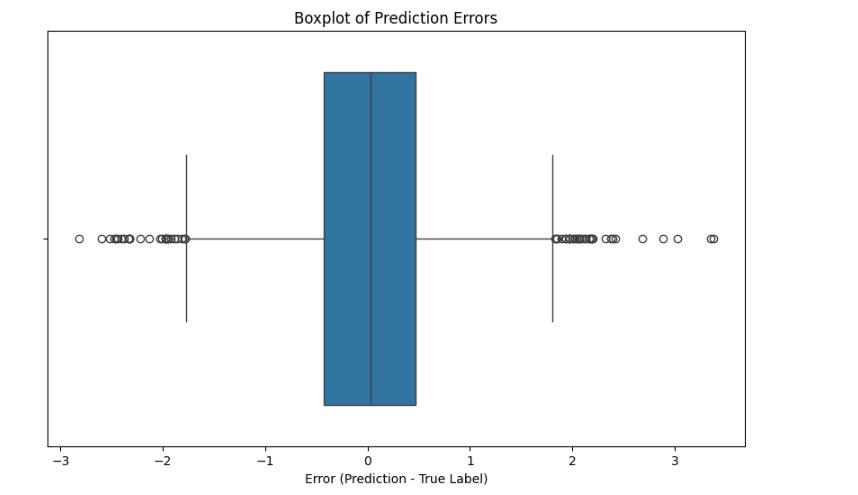
\includegraphics[width=0.8\textwidth]{ri4.png} 
\end{figure}


Ova slika ilustruje boxplot grešaka između predikcija modela i stvarnih vrednosti. Boxplot pokazuje da je medijana grešaka blizu nule, što sugeriše da model generalno dobro predviđa. Ipak, prisutni su outlajeri (udaljene tačke) na obe strane, što ukazuje na to da model u nekim situacijama pravi značajne greške. Ovi outlajeri mogu predstavljati neobične podatke ili sugerisati potrebu za dodatnim koracima u pretprocesiranju ili unapređenju modela.



\section{Klasterovanje korišćenjem transformera}

\subsection{Generisanje embedding-a}

\textbf{Embeddings} predstavljaju numeričke prikaze reči, fraza ili drugih entiteta u obliku vektora u višedimenzionalnom prostoru. Oni su ključni deo transformera, omogućavajući modelima da razumeju i obrađuju jezik na način sličan ljudskom razumevanju. Postoji nekoliko pristupa za generisanje embeddings-a u transformer modelima, u zavisnosti od specifičnog modela i primene. U projektu su prikazana dva načina.

\vspace{1em}
U modelima kao što je BERT, korišćenje \textbf{pooler\_output} omogućava dobijanje reprezentacije za ceo unos (npr. rečenicu), koja se često koristi za klasifikacione zadatke. Ovaj embedding služi kao ulaz za klasifikacione slojeve, omogućavajući modelu da donosi odluke na osnovu celine rečenice. Iako je \textbf{pooler\_output} jednostavan i efikasan za određene klasifikacione zadatke, \textbf{mean\_pooling} može pružiti bogatije i robusnije reprezentacije, što ga čini pogodnijim za zadatke gde su kontekst i detalji od ključne važnosti.

\newpage
\begin{figure}[h]
    \centering 
    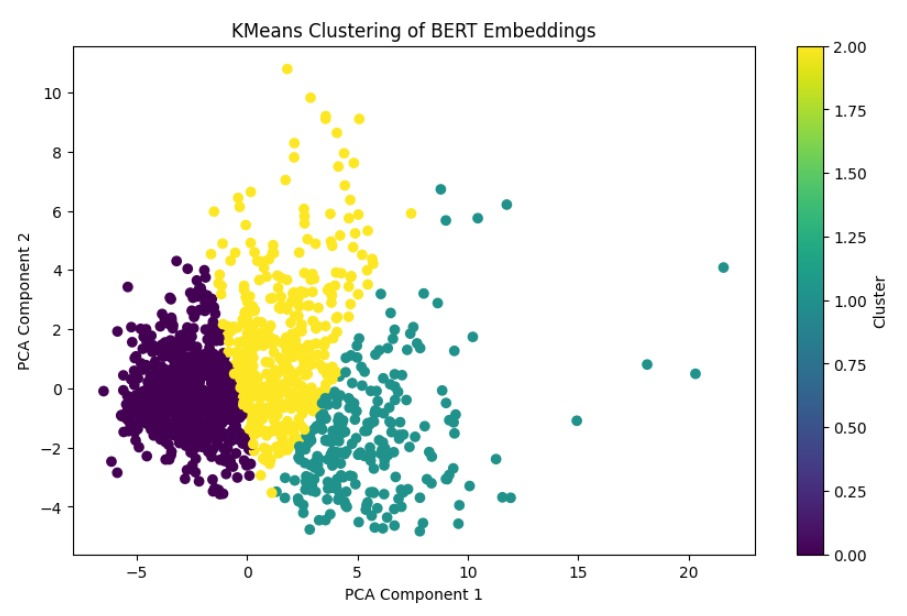
\includegraphics[width=0.8\textwidth]{ri5.jpeg} 
\end{figure}

Klasteri iz ovog koda su manje koherentni. To znači da rečenice koje su slične možda neće biti u istom klasteru.
\newline
\newline
\textbf{def get\_embeddings(input\_ids, attention\_mask)}: Ova linija definiše funkciju koja prima dva argumenta: input\_ids i attention\_mask. Ovi argumenti su ključni za tokenizovane ulaze koje BERT model zahteva.
\newline
\newline
\textbf{input\_ids} predstavljaju identifikatore tokena koji su dobijeni tokom tokenizacije rečenica. \textbf{attention\_mask} je binarni niz koji pokazuje koje tokene treba obraditi (1 za tokene koji se obrađuju i 0 za one koji se ignoriraju, kao što su padding tokeni).
\newline
\newline
Ovi ulazi se konvertuju u PyTorch tenzore koristeći torch.tensor(), a zatim se prebacuju na uređaj (CPU ili GPU) koristeći .to(device). Ovo osigurava da su podaci na istom uređaju kao i model, što je ključno za pravilno izvođenje.
\newline
\newline
\textbf{with torch.no\_grad():} Ova linija koristi kontekstualni menadžer torch.no\_grad(), koji onemogućava praćenje gradijenata. Ovo je važno tokom evaluacije modela jer ne želimo da se računaju gradijenti kada ne treniramo model, čime se štede resursi i smanjuje upotreba memorije.
\newline
\newline
\textbf{Izvršavanje modela:} Ovde se ulazi prosleđuju BERT modelu. model(**inputs) automatski prosleđuje input\_ids i attention\_mask kao argumente modelu. Rezultat outputs je objekat koji sadrži različite informacije o izlazu modela.
\newline
\newline
\textbf{Izvlacenje embedding-a:} outputs.pooler\_output sadrži embeddings za ulazne rečenice. Ovaj embedding predstavlja agregiranu reprezentaciju rečenice, koja se često koristi za zadatke klasifikacije ili sličnosti.

\newpage
Rezultat pooler\_output se generiše iz poslednjeg skrivenog stanja modela. Konkretno, uzima se izlaz za prvi token u sekvenci, koji se obično označava kao [CLS] (class token). Ovaj token je dizajniran da sakuplja informacije iz celokupne rečenice.
\newline
\newline
Korišćenjem \textbf{mean\_pooling}, uzimanjem prosečne vrednosti vektora svih tokena, moguće je obuhvatiti raznovrsne informacije i kontekstualne aspekte rečenice, smanjujući rizik od gubitka relevantnih informacija. \textbf{Mean\_pooling} se pokazuje posebno korisnim u zadacima gde je važno uzeti u obzir sve reči u rečenici, kao što su zadaci semantičke sličnosti, gde model treba da razume ukupni kontekst.


\vspace{3em}
\begin{figure}[h]
    \centering 
    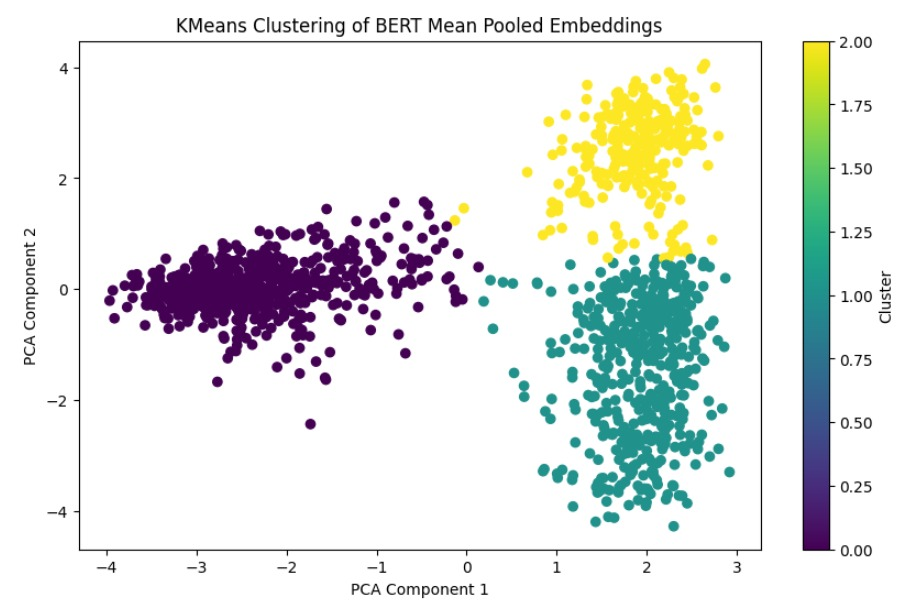
\includegraphics[width=0.8\textwidth]{ri6.jpeg} 
\end{figure}

Vidimo da ovaj pristup daje bolje rezultate u smislu koherencije klastera
često pokazuje bolje oblikovane klastere, sa jasnijim granicama između njih, što može sugerisati da je mean pooling uspešniji u identifikaciji sličnosti između rečenica.

\newline
\newline

\textbf{last\_hidden\_state = outputs.last\_hidden\_state}

Ova linija uzima poslednje skriveno stanje BERT modela, koje sadrži informacije o svakom tokenu u rečenici.
\newline
\newline
\textbf{Proširenje maske pažnje}: attention\_mask se proširuje kako bi se uskladio sa dimenzijama last\_hidden\_state. Ovo omogućava da se maska koristi za filtriranje skrivenih stanja.
\newline
\newline
\textbf{Suma skrivenih stanja}: Proizvod last\_hidden\_state * attention\_mask\_expanded osigurava da se samo skrivena stanja relevantnih tokena (onih koji nisu padding) sumiraju.
\newline
\newline
\textbf{Suma maske pažnje}: Ova suma broji koliko je aktivnih tokena bilo u svakoj rečenici, što je neophodno za izračunavanje proseka. Ova linija računa ukupan broj aktivnih (ne-padded) tokena u svakoj rečenici. Rezultat je vektor koji predstavlja koliko je aktivnih tokena bilo u svakoj rečenici.
\newline
\newline
\textbf{Mean pooling}: Konačno, mean pooled embedding se izračunava kao suma skrivenih stanja podeljena sa brojem aktivnih tokena, čime se dobijaju konačne reprezentacije rečenica.

Rezultat mean\_pooled je tensor dimenzija (batch\_size, hidden\_size), gde svaki red predstavlja prosečnu vrednost skrivenih stanja za odgovarajuću rečenicu, uzimajući u obzir samo aktivne tokene. To znači da svaka vrednost u mean\_pooled reprezentaciji obuhvata informacije o svim aktivnim tokenima, a ne samo o nekim pojedinačnim.
\newline
\newline


Osnovni pristup za izračunavanje sličnosti između rečenica korišćenjem \textbf{TF-IDF} vektorizacije i kosinusne sličnosti.




\begin{figure}[h]
    \centering 
    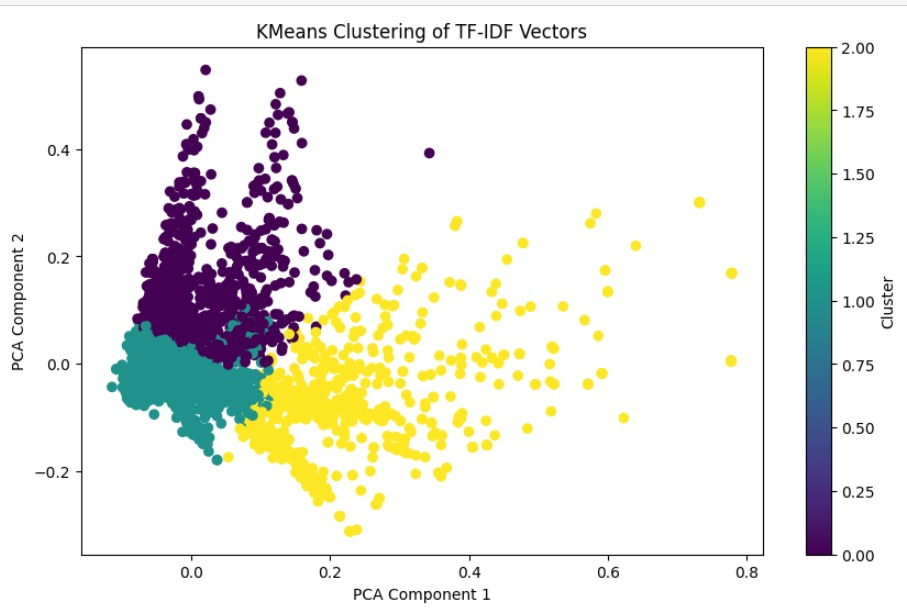
\includegraphics[width=0.8\textwidth]{ri7.jpeg} 
\end{figure}

Koristimo list comprehensions da iz train dataseta izvucemo rečenice. Pretpostavlja se da dataset sadrži ključ sentence1 za svaku stavku, pa se svaka rečenica čuva u listi sentences.
\newline
\newline

TfidfVectorizer je alat iz sklearn biblioteke koji transformiše tekstualne podatke u TF-IDF vektore. TF-IDF (Term Frequency-Inverse Document Frequency) je mera koja predstavlja važnost reči u odnosu na ceo korpus dokumenata.
\newline
\newline

Rezultat je matrica (tfidf\_matrix) u kojoj redovi predstavljaju rečenice, a kolone predstavljaju jedinstvene reči. Svaka ćelija sadrži TF-IDF vrednost koja pokazuje koliko je reč važna u toj rečenici.
\newline
\newline

Kosinusna sličnost meri sličnost između dva vektora (u ovom slučaju, rečenica) na osnovu ugla između njih. Ova linija računa kosinusnu sličnost između svih parova rečenica u tfidf\_matrix, i rezultat je matrica sličnosti (similarity\_matrix). Elementi matrice variraju od -1 (potpuna suprotnost) do 1 (potpuna sličnost).
\newline
\newline
\newline
\newline
\textbf{TF-IDF} pretvara rečenice u vektore na osnovu učestalosti reči u dokumentima. Ovaj pristup ne uzima u obzir kontekst i semantiku reči, već se fokusira na njihov značaj na osnovu učestalosti. Sličnosti se zasnivaju na broju pojavljivanja reči, što može dovesti do situacija u kojima rečenice koje su slične po značenju ne budu u istim klasterima. 
Klasteri nisu tako jasni i razdvojeni.

\end{document}
